\input{../templates/course_definitions}
% This Document contains the information about this course.

% Authors of the slides
\author{Tobias Hanf, Manik Khurana}

% Name of the Course
\institute{Java-Course}

% Fancy Logo
\titlegraphic{\hfill\includegraphics[height=1.25cm]{../templates/fsr_logo_cropped}}


\usepackage[style=british]{csquotes}
\usepackage{graphicx}

\def\signed #1{{\leavevmode\unskip\nobreak\hfil\penalty50\hskip1em
		\hbox{}\nobreak\hfill #1%
		\parfillskip=0pt \finalhyphendemerits=0 \endgraf}}

\newsavebox\mybox
\newenvironment{aquote}[1]
{\savebox\mybox{#1}\begin{quote}\openautoquote\hspace*{-.7ex}}
	{\unskip\closeautoquote\vspace*{1mm}\signed{\usebox\mybox}\end{quote}}

\title{Java}
\subtitle{Git}
\date{\today}


\lstdefinestyle{base}{
	%language=C,
	%emptylines=1,
	%breaklines=true,
	%basicstyle=\ttfamily\color{black},
	moredelim=**[is][\color{red}]{@}{@},
}


\begin{document}

% \section{Organisation}
\begin{frame}
	\titlepage
\end{frame}
\begin{frame}{Overview}
	\setbeamertemplate{section in toc}[sections numbered]
	\tableofcontents
\end{frame}

\section{Theory}
\begin{frame}{Git}
	\begin{aquote}{\url{https://git-scm.com/}}
		Git is a free and open source distributed version control system designed to handle everything from small to very large projects with speed and efficiency
	\end{aquote}
\end{frame}

\begin{frame}
	\begin{figure}
		\centering
		\def\svgwith{\columnwidth}
		\scalebox{0.55}{\input{git-storage.pdf_tex}}
		\caption{\url{https://eagain.net/articles/git-for-computer-scientists/}}
	\end{figure}
\end{frame}

\begin{frame}{Data}
	\begin{itemize}
		\item commit stores snapshot of data
		\item a commit can have one or more parent commits
		\item commits from an Directed Acyclic Graph (DAG)
		\item a commit can have a ''post-it''
	\end{itemize}
\end{frame}

\begin{frame}{Stages}
	\begin{figure}
		\centering
		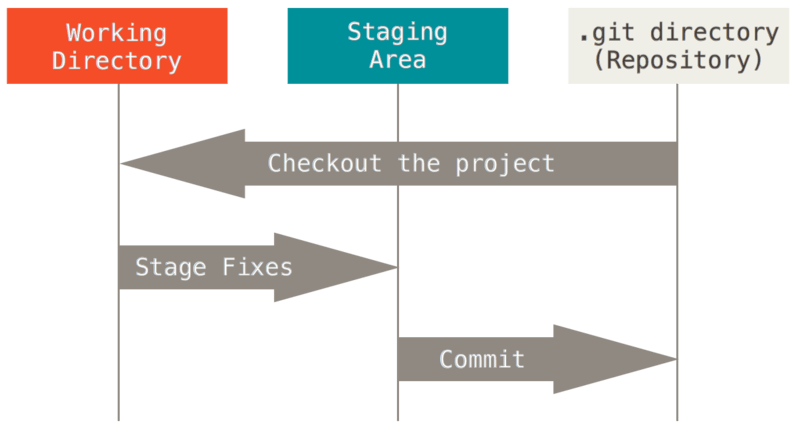
\includegraphics[width=\columnwidth]{10-git/areas.png}
		\caption{\url{https://git-scm.com/book/en/v2/images/areas.png}}
	\end{figure}
\end{frame}

\section{Branches}
\begin{frame}[fragile, allowframebreaks]{Branches}
	A Branch is a name ''referencing'' a commit. The current branch defines the position of the HEAD pointer.
	\vspace{2cm}
	
	Images taken from: \url{https://git-scm.com/book/en/v2/Git-Branching-Branches-in-a-Nutshell} 
	\framebreak
	\begin{figure}
		\centering
		\scalebox{0.9}{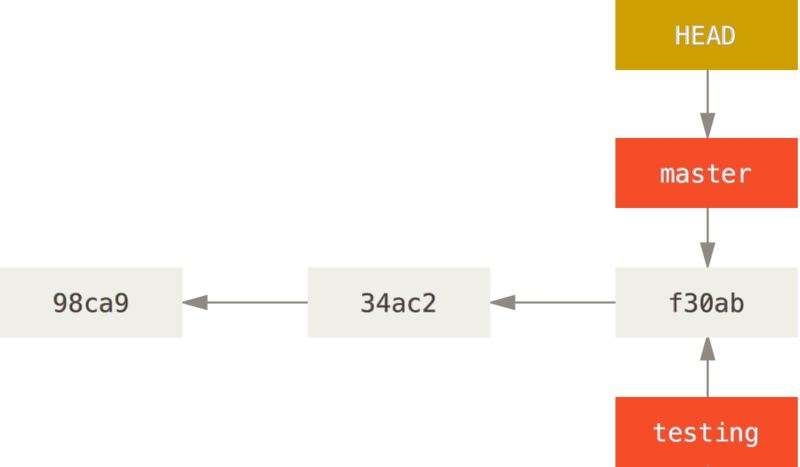
\includegraphics[width=\columnwidth]{10-git/head-to-master.png}}
		\caption{git checkout master}
	\end{figure}
	

	\framebreak
	\begin{figure}
		\centering
		\scalebox{0.9}{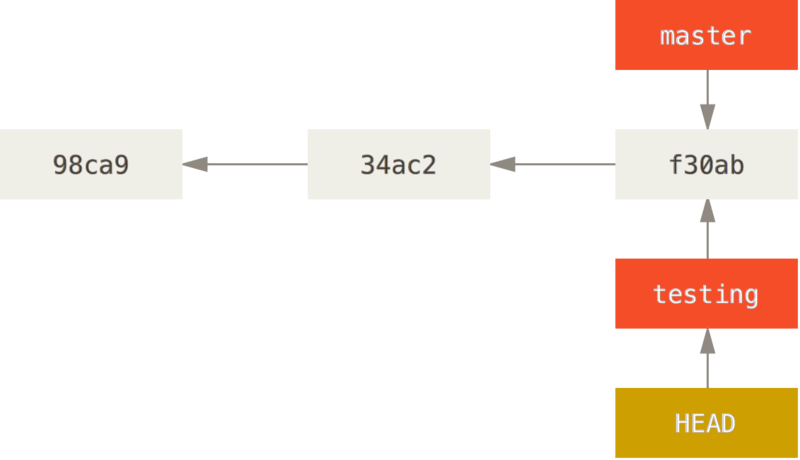
\includegraphics[width=\columnwidth]{10-git/head-to-testing.png}}
		\caption{git checkout testing}
	\end{figure}

	\framebreak
	\begin{figure}
		\centering
		\scalebox{0.9}{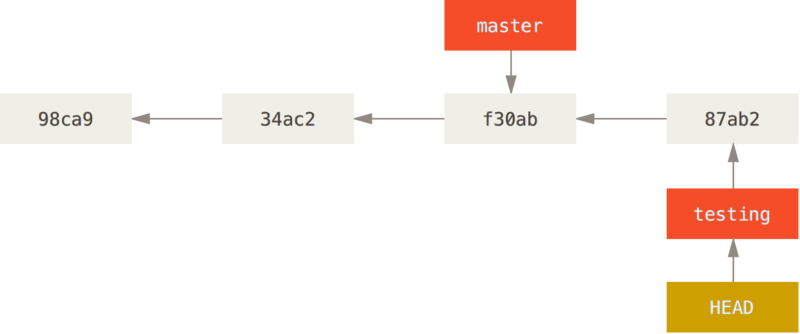
\includegraphics[width=\columnwidth]{10-git/advance-testing.png}}
		\caption{git commit -m 'something something'}
	\end{figure}

	\framebreak
	\begin{figure}
		\centering
		\scalebox{0.9}{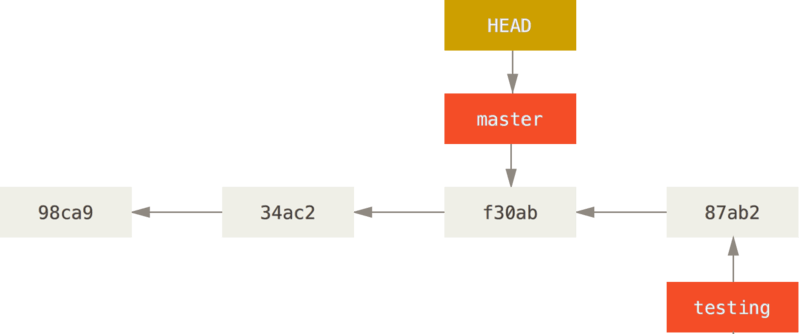
\includegraphics[width=\columnwidth]{10-git/checkout-master.png}}
		\caption{git checkout master}
	\end{figure}

	\framebreak
	\begin{figure}
		\centering
		\scalebox{0.9}{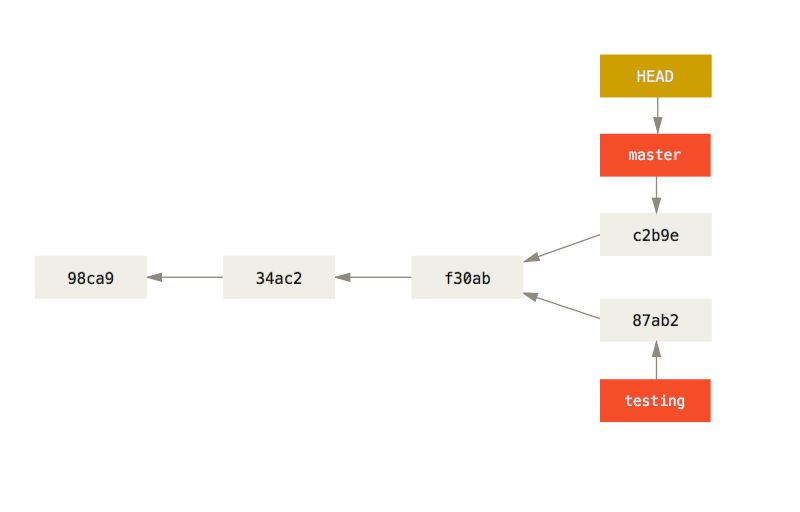
\includegraphics[width=\columnwidth]{10-git/advance-master.png}}
		\caption{git commit -m 'other things'}
	\end{figure}
	\framebreak
	
	Useful commands:
	\begin{itemize}
		\item Move  branch to different commit: \\ \texttt{git branch -f <branch-name> <new-tip-commit>}
		\item Create new branch and checkout: \\ \texttt{git checkout -b <branch-name>}
	\end{itemize}
\end{frame}
\begin{frame}[allowframebreaks]{Merging}
	Merging: combining two or more branches\\
	\begin{figure}
		\centering
		\scalebox{0.9}{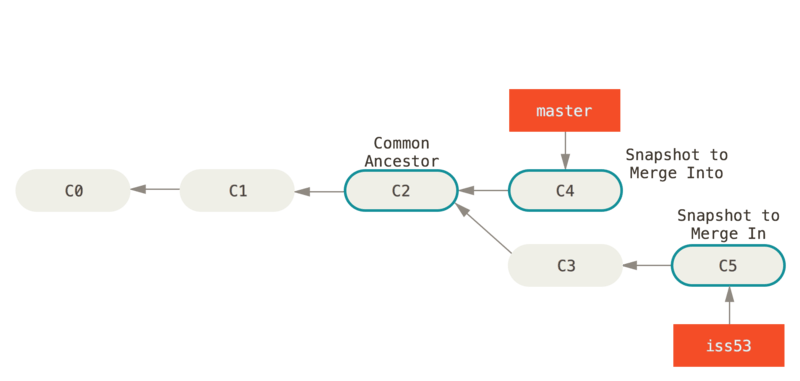
\includegraphics[width=\columnwidth]{10-git/basic-merging-1.png}}
		\caption{git checkout iss53}
	\end{figure}
\framebreak
	\begin{figure}
		\centering
		\scalebox{0.9}{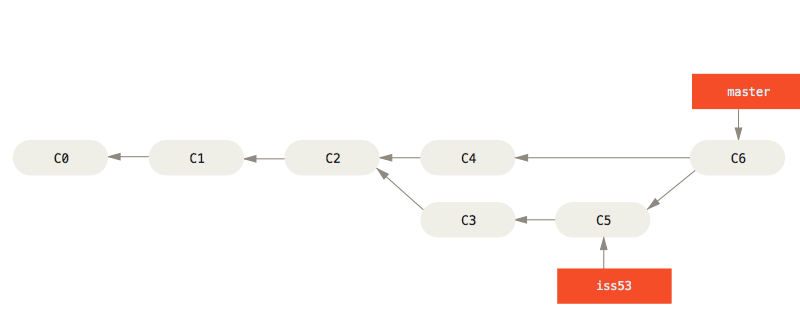
\includegraphics[width=\columnwidth]{10-git/basic-merging-2.png}}
		\caption{git checkout master; git merge iss53}
	\end{figure}
	\url{https://git-scm.com/book/en/v2/Git-Branching-Basic-Branching-and-Merging}
	
\end{frame}
\begin{frame}[allowframebreaks]{Rebaseing}
	Rebase: Moves commits from one branch (and the branch) onto the start of another
	\begin{figure}
		\centering
		\scalebox{0.9}{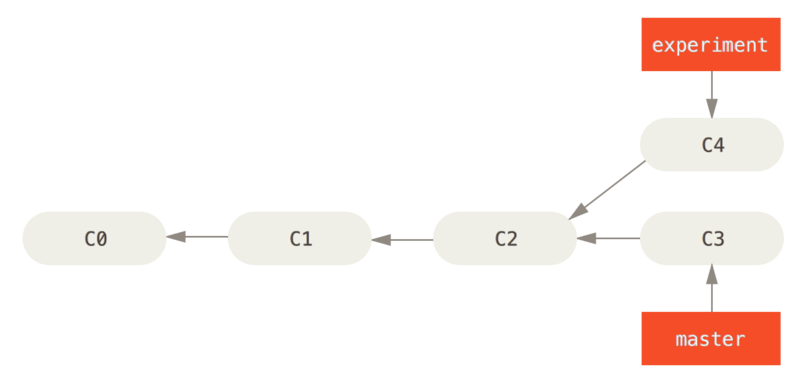
\includegraphics[width=\columnwidth]{10-git/basic-rebase-1.png}}
		\caption{git checkout experiment}
	\end{figure}

\begin{figure}
	\centering
	\scalebox{0.9}{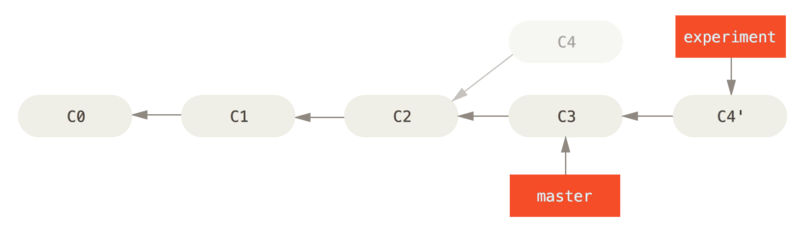
\includegraphics[width=\columnwidth]{10-git/basic-rebase-3.png}}
	\caption{git rebase master}
\end{figure}
\begin{figure}
	\centering
	\scalebox{0.9}{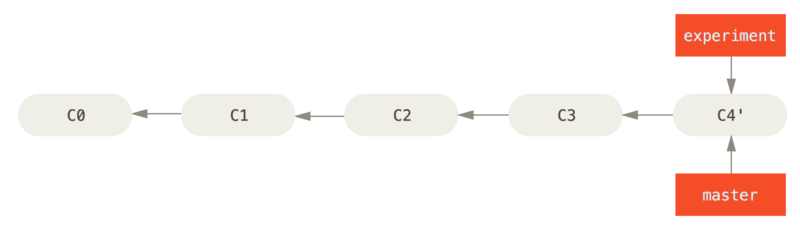
\includegraphics[width=\columnwidth]{10-git/basic-rebase-4.png}}
	\caption{git checkout master; git merge experiment}
\end{figure}
\url{https://git-scm.com/book/en/v2/Git-Branching-Rebasing}
	
\end{frame}
\begin{frame}{Cherry-Picking}
	\texttt{git cherry-pick <commit>}
	\begin{itemize}
		\item Cherry-Picking copy a specific commit to the branch
		\item can be handy
		\item but can lead to problems (duplicate commits)
		\item some people like it others not
	\end{itemize}
	
\end{frame}
\begin{frame}{Merge vs Rebase (vs FF-Merge)}
	\begin{columns}
	\begin{column}{0.5\textwidth}
		\centering
		Merge
		\begin{itemize}
			\item keeps history (non-destructive)
			\item more complicated structure
			\item every merge adds an extra commit
		\end{itemize}
	\end{column}
	\begin{column}{0.5\textwidth}
		\centering
		Rebase
		\begin{itemize}
			\item re-writes project history
			\item much cleaner history (structure)
			\item \textbf{never use it on public branches}
		\end{itemize}
	\end{column}
\end{columns}
\end{frame}
\begin{frame}[fragile, allowframebreaks]{Merge Conflict}
	\begin{figure}
		\centering
		\scalebox{0.685}{
\includegraphics[width=\columnwidth]{10-git/git-merge-without-conflict.jpg}}
		\caption{\url{https://webdevkin.ru/media/img/courses/git/meme/git-merge-without-conflict.jpg}}
	\end{figure}
	
	\framebreak
	
	Merge Conflict: occurs if you merge and two commits of different branches change the same part of a file.
	\begin{lstlisting}
		$: git merge conflict 
			Auto-merging second.txt
			CONFLICT (content): Merge conflict in second.txt
			Automatic merge failed; fix conflicts and then commit the result.
	\end{lstlisting}
	\framebreak
	The file on conflict will be changed to something like this
	\begin{lstlisting}
		$: cat second.txt 
			<<<<<<< HEAD
			First file
			=======
			Third file
			>>>>>>> conflict
	\end{lstlisting}
	Select what you want and remove everything else. Then add and commit.\\
	\texttt{git add second.txt}\\
	\texttt{git commit -m "Merge successful"}
\end{frame}
\section{Repositories}
\begin{frame}
	\begin{figure}
		\centering
		\scalebox{0.5}{
\includegraphics[width=\columnwidth]{10-git/git-xkcd.png}}
		\caption{\url{https://xkcd.com/1597/}}
	\end{figure}
\end{frame}
\begin{frame}[allowframebreaks]{Local vs Remote}
	\begin{itemize}
		\item git is a distributed VCS
		\item there is no \textbf{ONE} repository
		\item every one has a different version of a repository
		\item changes can be exchanged via a remote repository
		\item most errors occur while working with a remote repo
	\end{itemize}

	
	

	\framebreak
	
	
	To get a local copy of a remote repo: \texttt{git clone <repository-url>}\\
	\vspace{.5cm}
	Changes you make are only locally\\
	\vspace{.5cm}
	You have to explicitly \texttt{push} them to the remote repo.\\
	\vspace{.5cm}
	There are this a local and remote version for a remote branch in your local repo.\\
	\vspace{.5cm} 
	These remote versions have a special name: \texttt{origin/<branch-name>}
	
	
\end{frame}
\begin{frame}[allowframebreaks]{Fetch}
	
	\texttt{git fetch}: get all changes from the remote repository
	
	\begin{figure}
		\centering
		\scalebox{0.75}{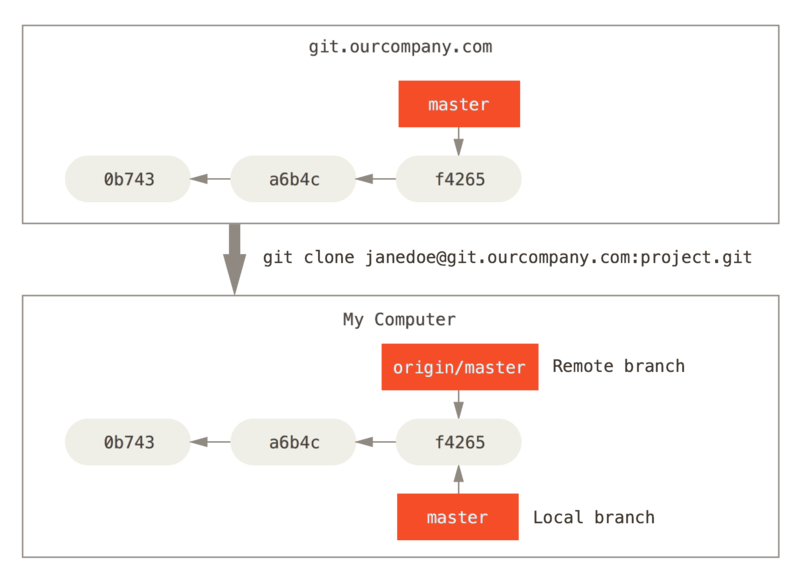
\includegraphics[width=\columnwidth]{10-git/remote-branches-1.png}}
	\end{figure}


	
	\begin{figure}
		\centering
		\scalebox{.9}{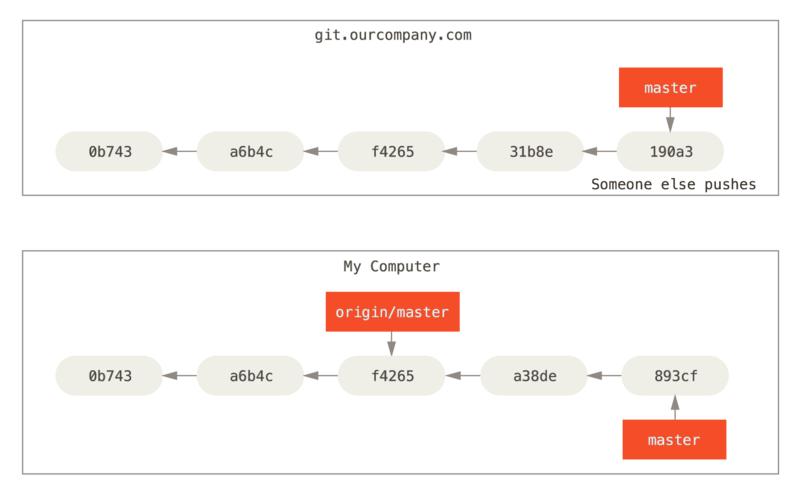
\includegraphics[width=\columnwidth]{10-git/remote-branches-2.png}}
		\caption{Add new commits to master}
	\end{figure}

\begin{figure}
	\centering
	\scalebox{0.8}{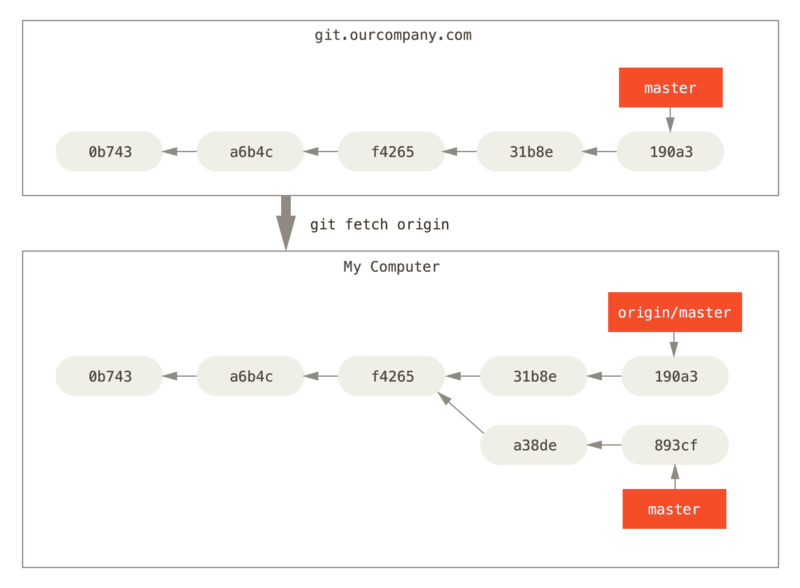
\includegraphics[width=\columnwidth]{10-git/remote-branches-3.png}}
	\caption{\texttt{git pull}}
\end{figure}

\end{frame}
\begin{frame}{Pull}
	Combines: \texttt{git fetch} und \texttt{git merge origin/<branch-name>}\\
	\vspace{1cm}
	Other option: \texttt{git merge --rebase}\\
	Does a rebase instead of a merge
\end{frame}
\begin{frame}[fragile]{Push}
	\texttt{git push}: pushes your locale changes to the remote repository\\
	\vspace{.5cm}
	For this to work all changes from the remote repo need to be in your local repo.
	\begin{lstlisting}[language=sh,basicstyle=\tiny]
		Pushing to ...
		To ...
		! [rejected]        master -> master (fetch first)
		error: failed to push some refs to '...'
		hint: Updates were rejected because the remote contains work that you do
		hint: not have locally. This is usually caused by another repository pushing
		hint: to the same ref. You may want to first integrate the remote changes
		hint: (e.g., 'git pull ...') before pushing again.
		hint: See the 'Note about fast-forwards' in 'git push --help' for details.
	\end{lstlisting}
\end{frame}
\begin{frame}{Saving your repo}
	\begin{itemize}
		\item \texttt{git checkout <branch>}: moves uncommited changes to branch
		\item \texttt{git stash}: saves current state of directory
		\item \texttt{git reset}: resets HEAD to specific state (removes commits)
		\item \texttt{git revert}: reverts existing commits by creating new commit
		\item \texttt{git blame}: see who fucked up (ruining friendships since 2005)
	\end{itemize}
\end{frame}
\begin{frame}{Submodules}
	A git repo can have other git repos as submodules
	\begin{itemize}
		\item Add submodule: \texttt{git submodule add <repo-url>}
		\item Commit add: \texttt{git commit -am 'Add submodule ...'}
		\item Push changes: \texttt{git push origin master}
	\end{itemize}
	Use a repo with submodules
	\begin{itemize}
		\item Get repo: \texttt{git clone <repo-url>}
		\item Init: \texttt{git submodule init}
		\item or: \texttt{git clone --recurse-submodules <repo-url>}
		\item update: \texttt{git submodule update --remote <module-repo-name>}
	\end{itemize}
\end{frame}
\section{Best Practice}
\begin{frame}{General}
	\begin{itemize}
		\item commit frequently, push often
		\item if there is a problem, keep calm (and use a search engine)
		\item use (a lot of) branches
		\item push only (semi) tested code
		\item use rebase for cleanups 
	\end{itemize}
\end{frame}
\begin{frame}{Commit messages}
	Read:  \url{https://cbea.ms/git-commit/}
	\begin{itemize}
		\item Subject should be 50 characters
		\item Capitalize Subject and use imperative mood
		\item wrap body at 72 chars
		\item explain the What and Why in body
	\end{itemize}
\end{frame}
\begin{frame}{branch strategies}
	Different strategies:
	\begin{itemize}
		\item only push tested code to main
		\item have development branch to merge features
		\item every feature/issue/bug should have its own branch
		\item these branches should be short lived
		\item don't work on branches with lots of outside changes
	\end{itemize}
\end{frame}
\begin{frame}{Gitlab/Github}
	\begin{itemize}
		\item learn git first
		\item use issues to communicate
		\item leverage Pull/Merge requests to add features
		\item master the concepts not the platform
	\end{itemize}
\end{frame}
\section{Link collection}
\begin{frame}
	\begin{itemize}
		\item \url{https://git-scm.com/docs}
		\item \url{https://git-scm.com/book/en/v2}
		\item \url{https://cbea.ms/git-commit/}
		\item \url{https://learngitbranching.js.org/}
		\item \url{https://stackoverflow.com/}
		\item \url{https://docs.github.com/en/get-started}
		\item \url{https://docs.gitlab.com/ee/topics/use_gitlab.html}
	\end{itemize}
\end{frame}
\end{document}
